\documentclass[11pt]{article}

\usepackage{graphicx}
\graphicspath{{images/}}

\title{Design of a Multichannel Digital PID Controller}
\author{Michael Adams}
\date{May 3, 2015}

\begin{document}
\maketitle

\section{Introduction}

This document describes the hardware and software design of a general
purpose, multichannel, digital PID control system. The system supports
eight concurrent locking channels with ADC inputs and user-configurable
DAC or DDS outputs. Each channel operates at a maximum rate of 100kHz.
Optional digital filtering stages may be activated at the cost of
reduced operational rates. Output processing stages enforce output
bounds and support optional output scaling. A custom Python graphical
interface allows for real time configuration of controller parameters
and monitoring of controller state.\\

Controller logic is described in Verilog and implemented on a Xilinx
Spartan 6 FPGA\@. The FPGA is mounted on a circuit board that contains
an 8-channel ADC (Analog Devices AD7608, 18-bit resolution, 200 ksps)
and an 8-channel DAC (Texas Instruments DAC8568, 16-bit resolution). The
board provides I/O ports for interfacing with external DDS chips.\\

A high level block diagram of the system is shown below in Fig. 1.  Up
to eight analog process variable signals are probed by the AD7608 chip.
Data is sampled at a rate of 200kHz and passed through a digital
first-order sinc filter on the AD7608. The filter oversamples at a rate
of 2x. The digitized and filtered signals are read by the ADC Controller
module at a rate of 100kHz over two serial interfaces. The ADC
Controller passes data into the PID pipeline, which computes the PID
sum. Data is finally routed to DDS or DAC controllers, depending on
configuration options. System parameters are set and state probed
through the FrontPanel Controller, which communicated via USB 2.0 link
with the Python GUI\@.\\

\begin{figure}[h]
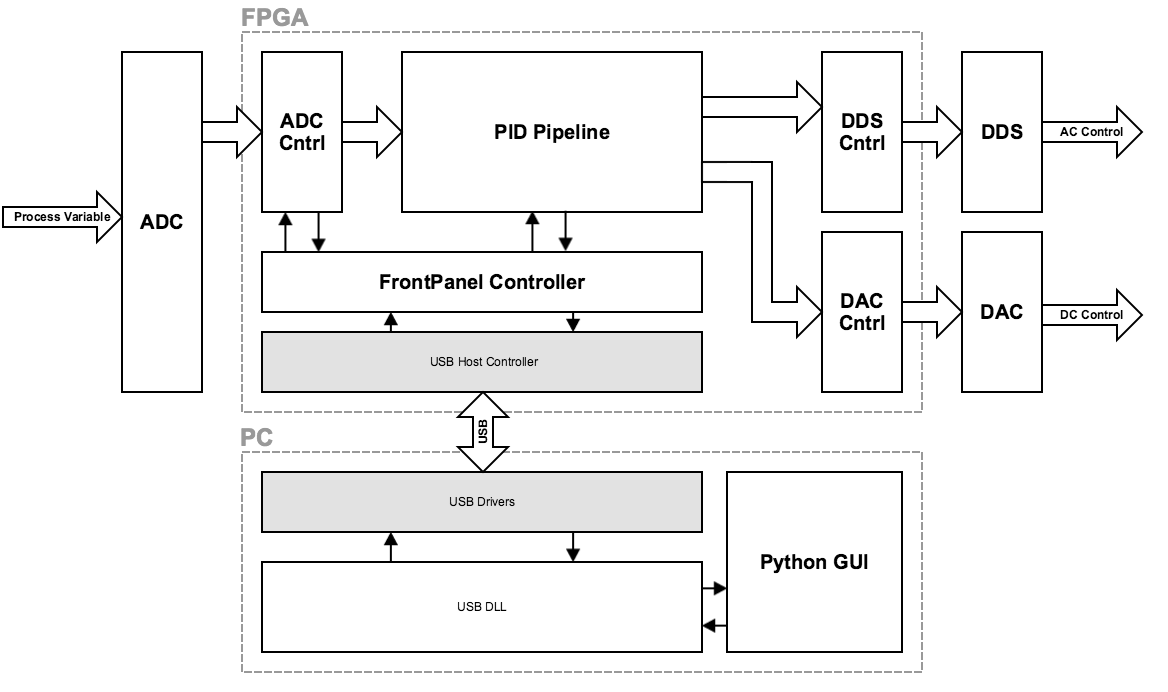
\includegraphics[width=\textwidth]{high_level_design}
\caption{High level PID controller block diagram}
\end{figure}

\section{Hardware Design}

\subsection{Overview}

Fig. 2 shows a block diagram of the controller hardware layout. Data
flows from left to right. The ADC Controller interfaces with the AD9912
chip, reading data over two serial interfaces at a rate of 100kHz. The
AD9912 and the ADC Controller run on a 17MHz clock. The rest of this
system runs at 50MHz. This clock boundary is bridged with the Clock
Synchronizer unit. The synchronized data is passed to the Moving
Average filtering stage, where it is optionally filtered according to
the system configuration. Data is then passed to the PID filtering stage
where the PID sum is computed. Data is then routed, according to
user-specification to either a DAC or DDS output preprocessor. This
stage enforces output bounds and optionally scales the output signal.
The final output signal is delivered via controller to either a DAC or
DDS chip.

\begin{figure}[h]
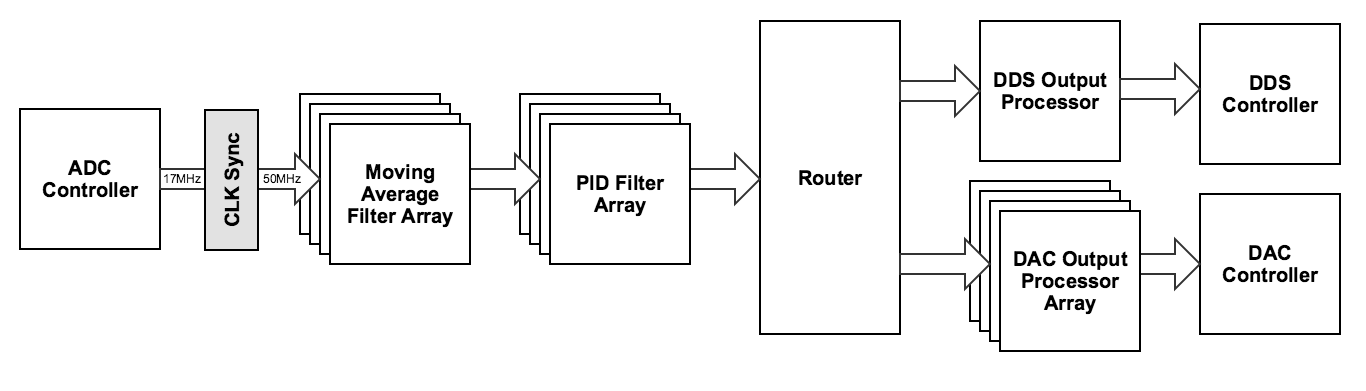
\includegraphics[width=\textwidth]{hardware_design}
\caption{Hardware block diagram.}
\end{figure}

\subsection{ADC Controller}

The ADC controller interfaces with the AD9912 chip and manages its
operation. Upon system reset, the ADC controller initiates the AD9912
for maximum-rate 200kHz continuous data sampling. In order to
achieve this rate, the ADC controller reads data from the AD9912
concurrently as it is converting new data. The ADC controller reads two
channels at a time over twin serial interfaces.

\subsection{Clock Synchronizer}

The AD9912 and ADC controller operate at 17MHz, while the rest of the
system operates at 50MHz. The clock synchronizer serves to bridge these
two clock domains. The clock synchronizer uses a finite state machine to
output a single 50MHz data valid pulse for every a single input 17MHz
data valid pulse.

\subsection{Moving Average Filter}

The moving average filter optionally maintains a moving average of its
input data stream. The oversampling rate for each filter-there is one
for each input ADC channel-is set in the Python GUI\@. The moving average
filter collects enough samples to satisfy the oversample rate,
computes the average of the collected data, and passes the average on to
the PID filter stage.

\subsection{PID Filter}

The PID filter stage computes the PID weighted sum according to
parameters set in the Python GUI\@. The filter includes overflow checking
and can be optionally deactivated.

\subsection{Router}

The router unit routes processed input data signals to the appropriate
output channel according to mappings set in the Python GUI\@. Any one of
the eight input channels can be mapped to any one of the output
channels. The router maintains an internal mapping table, pairing input
channel numbers with output channel numbers.

\subsection{Output Preprocessor}

The output processor stage enforce data bounds and apply an optional scaling
factor to the data stream before it is sent to the DAC or DDS chips. The
data bound and scaling factor are specified in the Python GUI\@. The
output preprocessor stage also conducts overflow checking.

\subsection{DAC/DDS Controllers}

The DAC and DDS controllers interface with external DAC and DDS chips
respectively, transmit the processed data stream via serial link. As the
DAC chip features 8 discrete output channels, the DAC controller manages
an internal write queue. The DDS chip only has on channel so the DDS
controller simply passes data straight through without any queuing. The
DAC and DDS controllers can easily be swapped with different components
if hardware is ever changed in the future to include different model DAC
or DDS chips.

\subsection{Frontpanel Controller}

The Frontpanel controller manages sending and receiving of data to and
from the Python GUI\@. The Frontpanel controller maintains three receive
Frontpanel data endpoints and one address endpoint to receive controller
configuration parameters. Data is sent to the data endpoints, and an
address specifying to the parameter type and channel number is sent to
the address endpoint.

\end{document}


